%
% Tesi D.S.I. - modello preso da
% Stanford University PhD thesis style -- modifications to the report style
%
%%%%%%%%%%%%%%%%%%%%%%%%%%%%%%%%%%%%%%%%%%%%%%%%%%%%%%%%%%%%%%%%%%%%%%%%%%%
%                                                                         %
%			TESI DOTTORATO                                                %
%			______________                                                %
%                                                                         %
%			AUTORE: Elena Pagani                                          %
%                                                                         %
%			Ultima revisione: 7.X.1998                                    %
%                                                                         %
%%%%%%%%%%%%%%%%%%%%%%%%%%%%%%%%%%%%%%%%%%%%%%%%%%%%%%%%%%%%%%%%%%%%%%%%%%%
%
%
\documentclass[12pt]{report}
%
% \includeonly{}
%
%			PREAMBOLO
%
\usepackage[a4paper]{geometry}
\usepackage{amssymb,amsmath,amsthm}
\usepackage{graphicx}
\graphicspath{ {./images/} }
\usepackage{url}
\usepackage{epsfig}
\usepackage[italian]{babel}
\usepackage{tesi}
\usepackage{indentfirst}
\usepackage{epigraph}
\usepackage{enumitem}
\usepackage{setspace}
\onehalfspacing                %% <--- Better use setspace
\setlist{noitemsep}
% per le accentate
\usepackage[utf8]{inputenc}
\usepackage{hyperref}


%Figure con bordo
\usepackage{float}
\floatstyle{boxed}
\restylefloat{figure}


%
\newtheorem{myteor}{Teorema}[section]
%
\newenvironment{teor}{\begin{myteor}\sl}{\end{myteor}}
%
%
%			TITOLO
%
\begin{document}
\title{Progettazione di un'applicazione e conseguenze di un approccio ``continuos refactoring''}
\author{Samuel Gomes Brandão}
\dept{Corso di Laurea in Informatica} 
\anno{2013-2014}
\matricola{803939}
\relatore{Prof. Carlo Bellettini}
%\correlatore{Dr. Richard STEVENS}

\beforepreface
\prefacesection{Dedica}
        {\hfill \Large {\sl Ai miei genitori Mônica e Zilmar}}

        {\hfill \Large {\sl Aos meus pais Mônica e Zilmar}}
% 
%			PREFAZIONE
%
\prefacesection{Prefazione}
Ciao! Ci vuole scrivere una prefazione!
%
%
%			ORGANIZZAZIONE
\section*{Organizzazione della tesi}
\label{organizzazione}
La tesi \`e organizzata come segue:
\begin{itemize}
\item nel Capitolo 1 ....
\end{itemize}
%
%			RINGRAZIAMENTI
%
\prefacesection{Ringraziamenti}
Vorrei ringraziare Paolo Venturi, Diego Costantino, 
e il prof. Dr. Carlo Bellettini. 
\afterpreface


% 
% 
%			CAPITOLO 1: iNTRODUZIONE
\chapter{Introduzione}
\label{cap1}

Spazi Unimi è il nome dato a un progetto per l'ottenimento di dati sugli spazi dell’Università degli Studi di Milano, sviluppato durante il Tirocinio Interno per la laurea triennale in Informatica all’UNIMI, da Samuel Gomes Brandão, Diego Costantino e Palo Venturi. L'idea nasce a partire dalle proposte del progetto Campus Sostenibile, promosso dall’UNIMI e dal Politecnico di Milano, e si sviluppa posteriormente in autonomia, sotto l'orientamento del Prof. Dr. Carlo Bellettini.

Il progetto parte con lo sviluppo di un'applicazione software con lo scopo principale di estrarre, validare e correggere dati ottenuti da diverse sorgenti, procedendo in seguito alla loro integrazione. I dati vengono mantenuti su un database da venir utilizzato per futuri progetti attraverso l'uso di una specifica Application Programming Interface (API) con architettura REST (Representational State Transfer). 

Le informazioni integrate riguardano la topologia e la destinazione d'uso degli edifici universitari e i loro spazi, con particolare importanza alla elaborazione e presentazione delle piante interne e localizzazione di stanze precise. In questo modo, siamo in grado di fornire accuratamente informazioni sulla localizzazione di palazzi, aule, o stanze a secondo della loro tipologia d'uso (bagni, biblioteca, sale studio, ecc).

In definitiva, tre sono stati i principali compiti del progetto:
\begin{itemize}
  \item Estrarre la topologia interna degli edifici universitari a partire dalle piantine edili.
  \item Integrare le diverse informazioni testuali (fogli elettronici, file CSV\footnote{Comma separated values - formato testuale in cui le informazioni vengono inserite utilizzando le virgole come separatori}) fornite dall'università e validarle.
  \item Associare le informazioni testuali alla topologia dei palazzi, identificando la localizzazione di stanze rilevanti e la categoria funzionale delle altre stanze.
\end{itemize}

Su questa relazione descrivo il processo di sviluppo della suddetta applicazione da zero, con particolare rilievo alla ricerca della buona progettazione e all'utilizzo di una modalità operativa che ho chiamato “continuos refactoring” \footnote{Si veda il capitolo \ref{cap3}}. Per quanto riguarda i compiti sopra, per motivi di brevità mi concentrerò di più sugli aspetti di estrazione dati dalle piantine edili.

% 
% 
%			CAPITOLO 2
\chapter{Attività Preliminari}
\label{cap2}

\epigraph{Experience is simply the name we give our mistakes}{Oscar Wilde}



La prima sfida per lo sviluppo di un progetto è quella di capire i requisiti e i problemi coinvolti. A seconda della tipologia di progetto, ciò può richiedere tempo e dedicazione considerevole. Molto spesso però il capire avviene soltanto durante lo sviluppo stesso: sono casi in cui la comprensione del problema avviene, contraddittoriamente, con la sua risoluzione.

Il nostro primo passo è stato quello di pensare ai casi d'uso che volevamo coprire con la nostra applicazione. Da questo punto abbiamo proceduto verso la comprensione dei dati e delle informazioni disponibili e la scelta delle tecnologie più adeguate per la loro elaborazione. Le sorgenti dati che dovevamo integrare erano due principali, a loro volta suddivise in più tipologie di informazione e formati di provenienza.

Dal dipartimento di Edilizia dell'UNIMI abbiamo ottenuto le piante architettoniche dei palazzi utilizzati dall'Università, in formato DWG - un formato file proprietario, e una serie di fogli elettronici con informazioni dettagliate sui palazzi e sulle loro stanze, in speciale quelle utilizzate per scopi didattici.

Abbiamo convertito questi file binari in formato DXF (formato testuale ``CAD-compatible'' ma comunque incomprensibile all'essere umano) utilizzando uno strumento gratuito, dato che era il formato richiesto dalla libreria dxfgrabber \footnote{Libreria \textit{opensource}, sorgente disponibile in https://bitbucket.org/mozman/dxfgrabber} che abbiamo utilizzato. La dimensione dei file arrivava facilmente all'ordine dei megabyte, con decine di migliaia di righe su ognuno, il che è ragionevole, se consideriamo che ogni file contiene, oltre al disegno delle stanze, una marea di informazioni imprescindibili al lavoro edile (misure, tubature, passaggio di elettricità, porte e finestre, scale, ascensori, sezioni, ecc).

\begin{figure}[h]
    \centering
    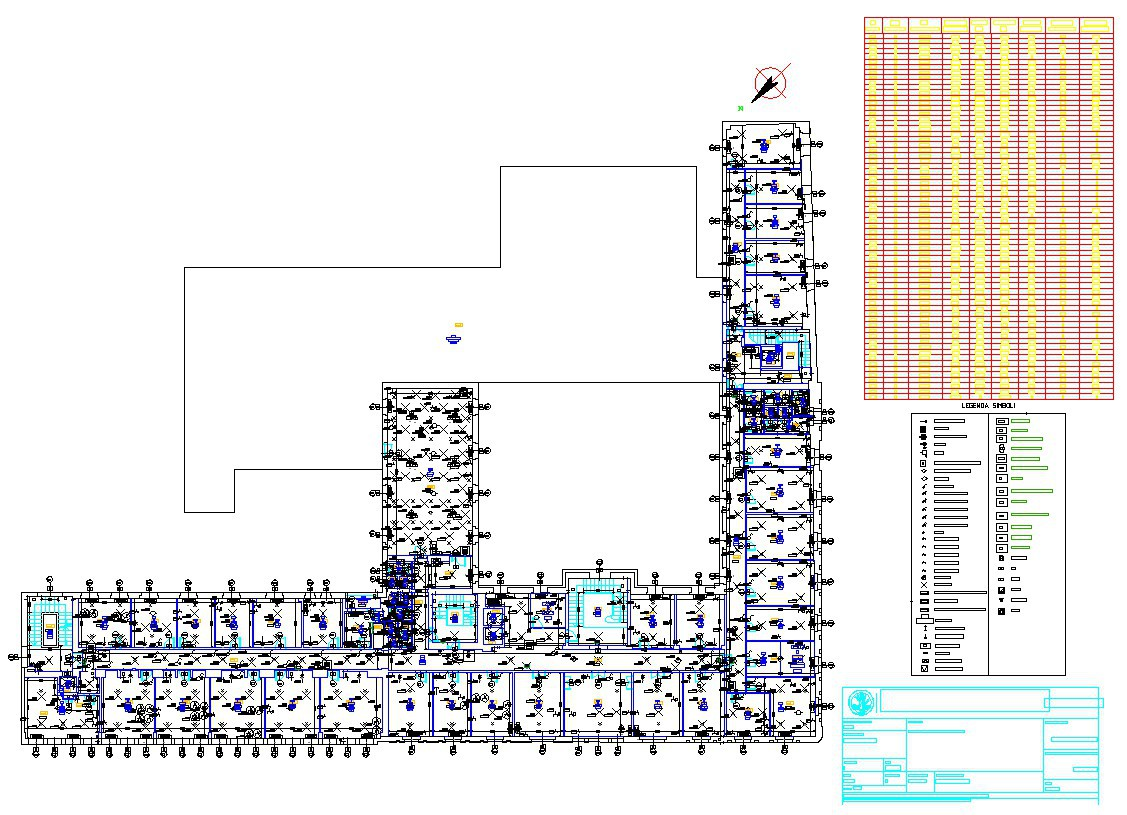
\includegraphics[width=\textwidth]{03-dxf-chaos.jpg}
    \caption{Esempio del contenuto di un file DWG di media complessità (Dipartimento di Informatica, 1º piano). La quantità di informazioni presente rende difficile la comprensione del contenuto informativo del file manualmente. }
    \label{fig:dxf_chaos}
\end{figure}

Con l'aiuto anche della divisione di Sistemi Informativi, rappresentata in speciale da Vincenzo Pupillo, abbiamo ottenuto in formato testuale CSV le informazioni utilizzate dal sistema Easyrooms, rispetto all'uso didattico degli spazi (eventi, lezioni, capienza delle aule, lauree, eccetera).

Entrambi i dipartimenti ci hanno aiutato con totale disponibilità e trasparenza, e senza il loro aiuto il nostro progetto non sarebbe mai stato portato a buon fine.

Con queste informazioni in mano ne abbiamo incominciato l'analisi, cercando di capire non solo le loro criticità, ma anche dove si sovrapponevano, completavano o fossero ridondanti. Al primo contatto ci sembravano perfette: avevamo informazioni di destinazione delle stanze, la loro capienza, accessibilità a disabili, e le potevamo localizzare sulle piante architettoniche utilizzando dei codici identificativi presenti anche su quelle. Dalle piante ottenevamo anche la localizzazione di aree di interesse come biblioteche, sale studio, bagni, spazi di ristorazione, eccetera.

In sostanza, il lavoro di integrazione consisteva nel far confluire in prima istanza i dati testuali dei dipartimenti di Sistemi Informativi e Edilizia. Si trattava allora di relazionare informazioni sui palazzi e sulle aule didattiche. Il risultato di questa operazione, dovevamo correlare con le informazioni presenti nelle piantine edili. Lo scopo finale è quello di avere un ulteriore set di dati disponibile, con la pretesa di essere più preciso e di averne più informazioni delle singole sorgenti di partenza.

\section{La consistenza dei dati}

Sotto uno sguardo più attento, però, l'immagine mentale che ci eravamo costruiti di quei dati incominciò a rilevare i suoi difetti: le fessure venivano come errori di battitura, l'utilizzo duplice di codici identificativi per i palazzi, piante architettoniche fuori scala o semplicemente disegno della stessa stanza più di una volta sullo stesso file. Spesso i disegni venivano ripetuti sulla stessa posizione, probabilmente frutto di un'operazione di copia e incolla interrotta a metà. All'occhio umano saltavano facilmente gli errori, e riuscivamo a correggerli riconoscendo dei pattern di riferimento, ma per un elaboratore no sarebbe stato così facile. Soltanto a un programmatore interessato ad estrarre informazioni in modo automatico con l'uso di un calcolatore questi errori avrebbero causato danni, e allora ci toccava gestirli.

Con buona probabilità questi errori sono stati accumulati lungo gli anni, ed è totalmente comprensibile che ci siano, se  consideriamo ad esempio che la maggior parte delle piante architettoniche di cui disponevano sono state disegnate in formato cartaceo e solo posteriormente trasferite in formato digitale, quando la costruzione dell'edificio era già finita. Sono inoltre state fatte e raccolte lungo periodi significativi, create da persone diverse, e perciò è difficile mantenere degli \textit{standard} nella loro rappresentazione digitale. Ovviamente nel processo di trasferimento da cartaceo a digitale dettagli vengono persi e errori vengono introdotti, e le versioni digitali non passano per la stessa meticolosa verifica di quelle utilizzate per la costruzione degli edifici. 

Da questo segue una nuova sfida: prima ancora di procedere all'integrazione, dovrebbe esserci un efficace meccanismo di validazione dei dati di partenza. Questo è diventato un ulteriore valore dell'applicazione, cioè la capacità di fornire un'analisi della correttezza sintattica dei file in input, permettendo un valido \textit{feedback} per ulteriori miglioramenti e correzioni manuali.

\section*{Nessuna assunzione}

La molle di dati era significativa, in speciale per i file DXF: più di 700, ognuno con dimensione media di 4.5Mb, e casi estremi di fino a 44Mb. Questi file contenevano tutte le informazioni edili: tubature, finestre, porte, scale, sezioni dei palazzi, disegno dei muri, cortili, terrazze, eccetera. Ci è stato poco tempo di analisi di quei dati per capire che l'unico modo di giudicarne la loro qualità sarebbe stato incominciando con la loro estrazione e imparando durante il processo. Queste caratteristiche hanno determinato tanti aspetti dello sviluppo, addirittura il nostro \textit{workflow}, che frequentemente si è dimostrato ``REPL Driven'' o ``Experimentation Driven''\footnote{Più dettagli nel capitolo \ref{cap3}}. 

Da queste analisi abbiamo concluso che potevamo fare poche o nessuna assunzione iniziale sulla qualità, formato, presenza o consistenza dei dati.

\section{Le scelte tecnologiche a partire dai dati}

Questa natura dei dati trasformava tante delle nostre richieste in \textit{``Wicked Problems''}, problemi la cui comprensione potrebbe avvenire soltanto durante la loro risoluzione stessa e non era possibile \textit{a priori}. Questo è stato uno dei primi motivi che ci ha fatto scegliere Python 3 come linguaggio di riferimento per l'estrazione e l'elaborazione: la capacità di scrivere velocemente degli script in grado di estrarre e produrre dettagliate analisi delle caratteristiche dei dati. 

Oltre a questo aspetto, anche i seguenti punti hanno contribuito alla scelta di Python:
\begin{itemize}
  \item La presenza delle \textit{list comprehentions}, un potente strumento per l'esecuzione di operazioni di trasformazione e filtraggio dei dati, specialmente se associate a funzioni per l'aggregazione di dati e agli iteratori di Python 3. Possiamo vedere le \textit{list comprehentions} come un'applicazione più leggibile del paradigma map-filter-reduce.
  \item L'esistenza di una forte comunità di sviluppatori e entusiasti per il linguaggio, specialmente in Italia.
  \item Ampia presenza di librerie di supporto per le attività che dovevamo eseguire (lettura delle piante, elaborazioni geometriche, generazione di immagini, ecc).
  \item Essendo Python un nuovo linguaggio per tutti i partecipanti al progetto, rappresentava una positiva sfida didattica.
  \item La scelta di Python non sarebbe limitante per la continuazione del progetto in futuro da parte di altri studenti/tesisti, in quanto è anche un linguaggio insegnato all'università.
\end{itemize}

Per quanto riguarda la scelta del DBMS (\textit{Database Management System}) è stata l'inconsistenza dei dati a guidare la scelta: le informazioni presenti sui diversi palazzi non erano omogenee in termini quantitativi ne qualitativi. Su qualche edifici disponevamo di più informazioni topologiche mentre su altri quasi nessuna. Anche le informazioni inerenti all'edificio stesso (come il suo nome rappresentativo o scopo d'utilizzo - ad esempio ``Dipartimento di Informatica'') non sempre erano presenti o valide, e ciò si ripeteva anche sugli altri dati. L'uso di un DBMS relazionale avrebbe portato a degli \textit{schema} con considerevoli campi \textit{null} e denormalizzato, due aspetti considerati \textit{anti-patterns} nella progettazione di \textit{database} relazionali. Per questi motivi abbiamo scelto un DBMS che seguisse un modello di memorizzazione \textit{schemaless}. 

Per le note caratteristiche prestazionali, supporto nativo a calcoli su coordinate geografiche, presenza di forte comunità, documentazione chiara e completa e la diversità di librerie aggiuntive disponibili, abbiamo scelto MongoDB come DBMS di riferimento.

% 
% 
%			CAPITOLO 3
\chapter{Svolgimento delle Attività}
\label{cap3}

Una mia particolare preoccupazione in fase iniziale del progetto, era quella di garantire la costante e ricorrente ricerca per la buona progettazione, prima, durante e dopo l'implementazione delle funzionalità. A parte i vantaggi ovvi per il prodotto finale di un approccio del genere, avevo lo scopo personale di sanare un mio \textit{gap} tecnico: sentivo che le mie conoscenze di (buona) progettazione del Software erano molto spesso di carattere teorico, e mi mancava allora l'assimilazione pratica dei principali concetti. Nella mia opinione l'esistenza di questo \textit{gap} è abbastanza comune tra gli altri studenti del mio stesso anno. Infatti, il perfezionamento di questo tipo di abilità può soltanto avvenire al confronto dello studio teorico con l'applicazione pratica, e in questo ho trovato un forte contributo nello sviluppo di questo lavoro.

In precedenza, nella mia carriera professionista e accademica, poche sono state le opportunità in cui ho potuto pensare al design del software complessivamente. Nella maggior parte dei casi, applichiamo precetti di design a livello \textit{micro}: singolo algoritmo, singola procedura, al massimo singola classe/modulo. Molto spesso neanche quello potevo fare, dato che la preoccupazione principale era quella di sintetizzare un algoritmo funzionante e performante, oppure di esplorare una determinata tecnica o risolvere un problema pratico in un determinato orizzonte temporale. Pensare invece a un sistema più complesso, con più componenti e elementi, organizzarli a vicenda, gestire le loro dipendenze, garantire un isolamento e disaccoppiamento salutare, non va fatto sotto stretti vincoli temporali, e allora non ha mai fatto parte della mia esperienza personale. 

La maggior parte della mia carriera professionista ha avuto luogo in ambito di sviluppo web, e dovevo sempre partire da un qualche \textit{framework}
\footnote{La maggior parte della mia carriera come sviluppatore ha avuto luogo utilizzando \textit{Ruby on Rails}, un \textit{framework} noto per non solo fornire una struttura MVC, ma per essere anche fortemente \textit{opinionated}, cioè di avere le \textit{best practices} definite e incentivate in modo molto chiaro.} 
o sistema preesistente, che mi dava già una risoluzione del \textit{design} a livello macro, di solito con l'utilizzo di pattern strutturali come MVC / MVP. A me restava più che altro rispettare le convenzioni fornite dall'ambiente di sviluppo e assicurarmi che a livello micro (metodi, classi) non causare troppi danni.

Su questo progetto non avevamo una struttura di partenza, e non avevamo qualcuno all'interno del \textit{team} che ci mostrasse le soluzioni migliori. In altre parole, la mancanza di esperienza nella costruzione del (buon) software da zero rappresentava una significativa sfida didattica e pratica su questo progetto.

\section{\textit{La scelta di un workflow: partire con il TDD}}

Per incominciare lo sviluppo avevamo l'obbiettivo di utilizzare il \textit{TDD - Test Driven Development}, un consacrato \textit{workflow} per lo sviluppo software noto per portare a soluzioni di design più semplici, pulite, disaccoppiate e testabili, tutte proprietà desiderabili da un software. Dato che sul TDD esiste già una svariata bibliografia online, lo riassumo in poche parole: consiste sostanzialmente nello scrivere i test delle nuove funzionalità prima di implementarle, seguendo un preciso flusso di lavoro (scrivo il test, lo eseguo e lo vedo fallire, implemento la funzionalità e rieseguo il test fino a farlo passare, faccio \textit{refactoring} e ricomincio con la prossima funzionalità). In questo modo è permesso allo sviluppatore testare l'interfaccia stessa delle funzioni, metodi, moduli o oggetti che dovrà sviluppare, per poi andare a riempire i dettagli.

Con questo obbiettivo in mente abbiamo incominciato il progetto affrontando quello che ci sembrava l'aspetto più difficile e che allo stesso tempo più ci interessava, cioè l'estrazione dei dati delle piante architettoniche. Dovevamo allora scoprire in che modo la libreria dxfgrabber ci poteva aiutare. Naturalmente, abbiamo aperto la REPL
\footnote{
  REPL - \textit{Read Eval Print Loop}. Si tratta di un ambiente di programmazione interattivo che ci permette di inserire comandi del rispettivo linguaggio di programmazione ed avere il risultato stampato in sequenza 
} 
di Python, e abbiamo incominciato ad esperimentare con la libreria e i dati.

La libreria dxfgrabber gestiva il compito di leggere i file da disco, interpretare le sue informazioni e restituirci un oggetto che rappresentasse il suo contenuto. Ci forniva la lista di entità grafiche/geometriche (linee, segmenti, cerchi, raggruppamenti di oggetti) e i testi, o etichette, tutto rispettando i 
\textit{layers}
  \footnote{
    I \textit{layers} sono strati diversi su cui gli elementi del file vengono collocati. Servono a raggruppare elementi diversi per scopo funzionale o semantico, come nell'esempio citato per le porte.
  }
con cui il file veniva organizzato. La grande maggioranza di questi file seguiva uno standard preciso per il \textit{naming} dei \textit{layers}: c'era un \textit{layer} ``PORTE'', un \textit{layer} ``RM\$'' che conteneva i poligoni delle stanze, un \textit{layer} ``FINESTRE'', e così via. Ma in qualche file, Il layer ``PORTE'' potrebbe chiamarsi ``PORTA'', le finestre potrebbero essere state inserite insieme alle murature nel \textit{layer} ``MURI'', mentre il \textit{layer} ``SCALE'' era vuoto con le scale disegnate insieme alle stanze su ``RM\$''. Sul \textit{layer} delle porte, a volte trovavamo le porte disegnate come linee e archi sparsi, a volte raggruppate all'interno di oggetti composti (chiamati Insert, una specie di gruppo di oggetti), e lo stesso valeva per le finestre e le scale. 

Con morfologie talmente eterogenee da trattare, in che modo avremmo potuto incominciare il lavoro su questi dati/file utilizzando il TDD? Una delle qualità del TDD sta nel fatto che molto spesso, quando non si sa come incominciare l'implementazione di una funzionalità, si è in grado di scrivere almeno i test che andranno a testarla. Nel nostro caso, anche se studiassimo i dati a lungo, che assunzioni potevamo veramente fare? E allora che tipologia di test avremmo potuto scrivere inizialmente per guidarci lo sviluppo? Con queste domande abbiamo concluso che l'applicazione sistematica del TDD avrebbe portato all'utilizzo di almeno una delle seguenti strategie per la scrittura dei test iniziali:

\begin{itemize}
  \item Basarsi sui file VERI, rischiando di ottenere implementazioni che funzionassero soltanto per casi simili, suite di test troppo lenti test poco affidabili.
  \item Basarsi su una quantità enorme di dati fittizi, cercando di coprire molti casi, ma scrivendo dei test fragili e potenzialmente più numerosi di quanto fosse ragionevole, specialmente per la loro manutenzione.
  \item Basarsi su usi complessi di \textit{mock} per limitare la quantità di dati fittizi e isolare piccoli casi da trattare. Poco pratico perché i piccoli casi da trattare continuavano ad aumentare a seconda che esploravamo più file.
\end{itemize}

Per evitarle dovevamo essere in grado di fare qualche assunzione, ma non riuscivamo a trovare proprietà che venissero rispettate nel 100\% dei casi. Abbiamo capito un aspetto imprescindibile per un lavoro così complicato, su dati così eterogenei: non dovevamo cercare il 100\%. Non l'avremmo mai raggiunto. Ci serviva, invece, una soglia ammissibile di errore, la possibilità di segnalarli all'utente o superarli attraverso qualche euristica particolare. Sorsero allora i seguenti obbiettivi, per ogni funzionalità / problema in considerazione: 

\begin{itemize}
  \item Definire la soglia di errore ammissibile.
  \item Superare la maggior parte possibile di errori, con uso di euristiche diverse per coprire più casi possibili.
  \item Rilevare errori non risolubili per rendere possibile all'utente la loro correzione manuale. In questo modo, anche se non riuscivamo a soddisfare la soglia di errore ammissibile, avremmo sviluppato un sistema che tende in futuro a migliorare.
\end{itemize}

In altre parole, non avremmo più partito dai test, ma da un'esplorazione sistematica del problema e dei dati, e infatti era esattamente quello che avevamo già fatto alla prima apertura della REPL per l'esplorazione della libreria utilizzata: volevamo capire meglio in che modo lo strumento ci potrebbe aiutare nella gestione dei dati. Tale approccio ci ha consentito gestire meglio l'incertezza, sostituendo le assunzioni per ipotesi da testare.

In uno \textit{speech} nell'Agile UX NYC 2012, Joshua Seiden discorre sul rimpiazzare i \textit{requirements} con ipotesi quando sviluppando per un ambiente caratterizzato dall'incertezza: \textit{``When you\'re in production, building to known standard, you want requirements. When you\'re in an environment of uncertainty, you want hypotheses.''} (Seiden, 2012).

L'autore sottolinea che molto spesso i \textit{requirements} nascondono forti assunzioni sugli effetti dei cambiamenti, e la tecnica suggerita di esprimerli in forma di ipotesi è utile nell'esplicitare l'incertezza. Un approccio simile abbiamo adottato nel gestire le assunzioni che facevamo sui nostri dati, attraverso la definizione di soglie di errore come delle ipotesi di soddisfacibilità dei nostri requisiti.

In seguito allo stabilire delle ipotesi sui dati, seguiva la fase della loro validazione, dalla quale volevamo ricavare un percentuale di soddisfacibilità (quale percentuale dei dati totali soddisfa positivamente o negativamente l'ipotesi in questione).

\section{\textit{Experimentation Driven Development}}

Per \textit{Experimentation Driven Development} intendo una modalità pratica di sviluppo del \textit{software} che attraverso l'esplorazione pratica del dominio applicativo, dei problemi da risolvere, e della natura dei dati, si prefigge di:

\begin{enumerate}
	\item Garantire una comprensione più approfondita del problema.
	\item Capire caratteristiche importanti/comuni su una molle considerevole di dati.
  \item Rivelare in che modo il linguaggio utilizzato, i suoi moduli o librerie esterne possono contribuire alla risoluzione del problema
  \item Confrontare ipotetiche soluzioni con grandi quantità di input non fittizi per capirne la precisione e/o \textit{recall}.
	\item Permettere una naturale validazione e conseguente migrazione degli approcci di esplorazione utilizzati verso un'implementazione funzionante.
\end{enumerate}

È imprescindibile che l'esplorazione avvenga nell'ambiente stesso su cui avverrà l'implementazione. Per questo motivo abbiamo utilizzato la REPL, con l'interprete python bpython\footnote{\url{http://www.bpython-interpreter.org/}}, che fornisce diverse funzionalità utili per un approccio del genere:

\begin{itemize}
  \item Colorazione del codice per facilitarne la comprensione
  \item \textit{Indenting} automatico, il che risparmia considerevole tempo scrivendo codice su Python, in cui l'indentazione è significativa.
  \item Introspezione sui metodi e funzioni utilizzate, esibendo direttamente sulla REPL dettagli sulla loro segnatura e anche documentazione (docstring).
  \item Possibilità di salvare il codice utilizzato direttamente sul filesystem
  \item Funzionalità \textit{rewind}, che permette di disfare le istruzioni precedenti. Ci permetteva ad esempio di esplorare e trasformare i dati per vederne determinati risultati, tornare in dietro e riprovare con strategie diverse.
\end{itemize}

Il nostro \textit{workflow} basico era composto dai seguenti passi, eseguiti in modo iterativo:

\begin{itemize}
	\item Comprendere teoricamente la natura del problema
	\item Utilizzare la REPL per conoscere meglio i dati e le sfide implementative, analizzando la numerosità totale degli input e la quantità di casi che soddisfano  qualche insieme di proprietà desiderate.
	\item Creare/salvare codice che permetta o la risoluzione del problema (in termini di soglie ammissibili) o l'esecuzione di test significativi sulle funzionalità da implementare.
\end{itemize}

Ad ogni iterazione, le prove precedenti e codici ottenuti venivano riutilizzati e permettevano una più ampia comprensione, oltre a generare dei prototipi/bozze implementativi.

Il prototipo/bozza differisce da una versione finale a volte per aspetti di completezza (può non gestire ad esempio casi limite), a volte per qualità del codice o prestazioni (viene scritto il più veloce possibile in modo da non bloccare il \textit{workflow}, ma non necessariamente si tratta di un'implementazione efficace o chiara).

Non abbiamo scelto esplicitamente nessuna di queste metodologie di lavoro, piuttosto ci siamo fatti guidare dalla natura dei problemi e dei dati da trattare. 

\section*{\textit{Esempi pratici}}

Un esempio su cui abbiamo utilizzato questa strategia è l'estrazione delle stanze, e in seguito le etichette e testi associati a loro, in modo da poter identificare, ad esempio, dove si trovasse la ``Aula Beta'' sulla piantina, o quali stanze rappresentavano dei Bagni, studi o uffici, cioè le categorie delle stanze.

La lettura delle stanze è stata poco problematica, e con l'uso della REPL siamo riusciti a ottenere a piccoli passi i codici per estrarre le stanze e le etichette. Si noti che con la REPL partivamo alla esplorazione, mirando a una comprensione maggiore del problema e dei dati, e finivamo per risolvere il problema. In questo modo non era più possibile scrivere i test \textit{a priori}, invalidando uno dei punti cardine dell'uso sistematico del TDD.

Le difficoltà maggiori sono sorte nell'associare le etichette alle relative stanze. L'unico vincolo fra le etichette di una stanza e il suo disegno era la loro relativa posizione, senza nessun vincolo a livello sintattico. Abbiamo allora utilizzato un algoritmo che, dato un poligono S (stanza) e un punto P nello spazio (punto di ancoraggio dell'etichetta testuale), rispondeva alla domanda ``Il punto P è dentro il poligono S?''. Si tratta di un algoritmo particolarmente interessante e concettualmente semplice, chiamato \textit{Ray Casting Algorithm}\footnote{Una chiara spiegazione è presente su Wikipedia: \url{http://en.wikipedia.org/wiki/Point_in_polygon\#Ray_casting_algorithm}}.

La nostra ipotesi sui dati era che, essendo in grado di rispondere a questa domanda, saremmo riusciti ad associare etichette correttamente al 90\% delle stanze\footnote{La scelta di questa soglia era giustificata dal fatto che in mezzo ai file di cui disponevamo c'erano anche altri file che non ci davano informazioni utili, o che si riferivano a palazzi non utilizzati per scopi didattici, in cui la percentuale di identificazione di stanze sarebbe naturalmente più bassa}.

In presenza di stanze piccole o strette (come corridoi ad esempio), poteva capitare che l'etichetta, per mancanza di spazio, venisse collocata all'interno di una stanza vicina. All'occhio umano era semplice capire a quale stanza tale etichetta appartenesse, ma un po' più complicato in termini algoritmici.

\begin{figure}[h]
    \centering
    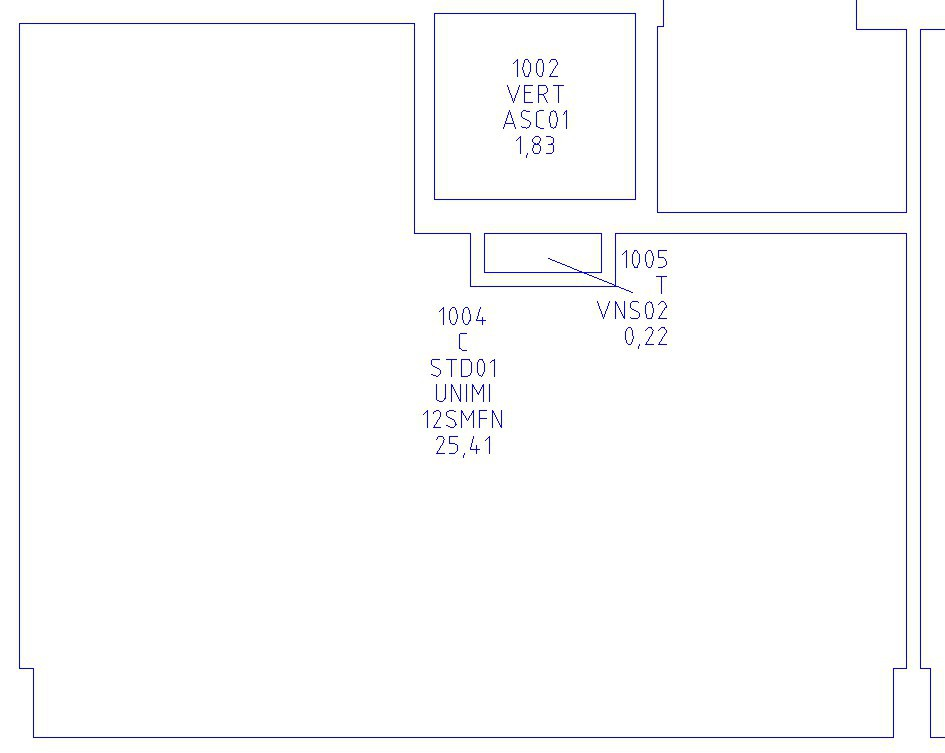
\includegraphics[width=300pt]{03-dxf-stanza-etichette-fuori.jpg}
    \caption{Esempio di stanza con più etichette al suo interno. Le etichette corrette sarebbero quelle indicate dal numero 1004. Quelle di numero 1005 sono riferite al piccolo rettangolo indicato (in questo particolare caso, ma non sempre) dalla linea uscente, e si tratta di un ``Cavedio Porta Impianti'', cioè uno spazio per il passaggio dei cavi}
    \label{fig:dxf_chaos}
\end{figure}

In seguito la REPL ci ha permesso di capire quanto buona effettivamente fosse la nostra soluzione. L'algoritmo riusciva ad associare etichette con un \textit{recall} del 94\% delle stanze, con una \textit{precision} sul 89\%. Avevamo in mano, dall'uso della REPL, una soluzione che sembrava quasi soddisfacente. Non avevamo il 90\% desiderato ma eravamo abbastanza vicini. 

Abbiamo allora lanciato una nuova ipotesi: se scartiamo qualche tipologie specifiche di stanze che ai nostri scopi sono di minore importanza, riusciremo ad aumentare la precisione relativa al 90\% desiderato, al patto di ridurre il percentuale di \textit{recall}.

Con l'uso della REPL abbiamo eseguito delle prove veloci manipolando i codici già esistenti in modo che scartassero soltanto le etichette di tipo ``cavedio'' e infatti siamo arrivati a un' \textit{recall} del 93\% con 90\% di precisione stimata.

Infatti, durante lo sviluppo, l'uso della REPL per l'esplorazione di questi dati prima dell'effettiva sintesi degli algoritmi e scrittura del codice ci ha permesso di affrontare i problemi in modo più efficiente. Ci permetteva velocemente di capire caratteristiche comuni o analizzare attributi dei dati e provare alternative, per poi migrare quelle conclusioni verso un'implementazione effettiva. Creando ipotesi, dimostrando che coprissero i casi prevalenti e aggiungendo in seguito euristiche per l'inclusione di più casi specifici, siamo riusciti ad affrontare la maggior parte delle difficoltà.

A volte ottenevamo dalla REPL un modulo già semilavorato, a volte semplicemente una media campionaria che ci permetteva di avere più confidenza nelle scelte prese.
Quando una precisione assoluta e deterministica non era possibile, l'analisi delle qualità dei dati giustificava assunzioni che ci permettevano di procedere a un'estrazione \textbf{sufficientemente o statisticamente buona}, superando la difficoltà di correggere errori umani. In altre parole, ci permetteva di continuare anche quando in termini assoluti sarebbe stato sbagliato farlo.

L'ultimo vantaggio di questa metodologia è quello di garantire un rapido \textit{feedback} per le strategie adottate. Di certo non tanto rapido quanto una suite di test, ma nel contesto in cui la scrittura dei test sarebbe stata problematica, l'uso della REPL ha agevolato significativamente la valutazione manuale e l'ottenimento di statistiche.

Un altro contesto in cui l'analisi statistica dei dati e dei file è stata essenziale è stato durante la fase di integrazione di informazioni sulle stanze e piani di ogni edificio. Alla fine della lettura e estrazione, abbiamo scoperto che non esisteva nessun standard identificativo per i piani che venisse rispettato da tutte le sorgenti. Non c'era un modo diretto per associare due piani dello stesso palazzo su sorgenti diverse, e ciò rendeva l'integrazione dell'informazione delle stanze molto difficile. La difficoltà era quella di dire quale piano di una determinata sorgente dovrebbe coincidere con quale piano di un altra sorgente. 

Con l'aiuto della REPL abbiamo scoperto che molto spesso determinate sorgenti avevano informazioni su piani che altre sorgenti non conoscevano, o che addirittura Easyroom colassava nel piano terra spesso stanze del piano sotterraneo e del piano terra. Queste caratteristiche creavano degli ostacoli per l'associazione dei piani fra le diverse sorgenti.

La REPL ci ha permesso anche di stabilire che su un impressionante 99\% dei piani era possibile trovare almeno una stanza, utilizzando il suo codice identificativo, che venisse rintracciata in tutte e tre sorgenti (piantine, informazioni testuali dell'edilizia e informazioni testuali di Easyroom), e allora la presenza di quella stanza ci dava un'informazione ortogonale ai piani delle diverse sorgenti. Sapendo in quale piano una stanza veniva rimappata per sorgente ci dava una forte indicazione di come quei piani dovrebbero venir relazionati. L'unico problema che rimaneva erano i casi estremi, in cui due stanze di uno stesso piano su una sorgente venivano rimappate su piani diversi in un'altra sorgente, o quando per qualche piano nessuna associazione di stanza con le altre sorgenti era possibile. L'algoritmo finale che abbiamo concepito gestisce tutti i possibili casi, e se ne accorge quando non riesce a trovare un'associazione fra piani di due o più sorgenti. 

In questo modo all'utente vengono segnalati i conflitti, sia quelli che abbiamo risolto in modo automatico che quelli la cui risoluzione non è possibile. Con l'uso di questa strategia e una serie di eurisitche per renderla più efficiente, siamo stati in grado di associare il 99\% dei piani correttamente. L'1\% che avanza è costituito da precisamente tre casi, due dei quali si presenta solo a causa di un errore di battitura dei dati originali (stanze identificate in modo sbagliato), e comunque vengono tutti e tre segnalati per la revisione dell'utente. 


\section{La naturale migrazione verso un approccio prototipale}

Molti componenti dell'applicazione finale sono nati a partire da questi esperimenti con la REPL, incentivando un approccio alla progettazione di tipo prototipale. 

Il principale vantaggio era quello di poter conoscere la natura dei problemi o i limiti e le potenzialità delle nostre scelte algoritmiche, senza dover pagare un prezzo troppo alto se mai fosse necessario tornare in dietro. Fino a questo punto non si trattava di design di software, ma di sola esplorazione e comprensione. A misura che riuscivamo ad avere implementazioni soddisfacenti per ogni funzionalità, le incorporavamo al \textit{codebase} principale e proseguivamo verso l'esplorazione di ulteriori limiti e possibilità.

Da queste versioni prototipali ottenute dalla sperimentazione, ottenevamo versioni più elaborate eseguendo delle continue trasformazioni e operazioni di \textit{refactoring}. Perché funzionasse correttamente, le prove sulla REPL dovevano essere estremamente veloci, e allora le attività di design e \textit{testing} non erano la priorità. In questa fase di \textit{refactoring} dovevamo sanare queste eventuali deficienze.

Col il nostro obbiettivo per la ricerca continua della buona progettazione, una volta capito meglio il \textit{wicked problem} in questione, lo sviluppo doveva proseguire in una di due possibili strade: scartare il prototipo per rifarlo da capo, o rielaborarlo. Mantenere la versione originale senza ripulirla e testarla non era una scelta possibile, specialmente a lungo termine. 

Dati i tempi stretti, nella maggior parte dei casi abbiamo optato per la rielaborazione del prototipo esistente e non per il suo scarto, poiché era evidente che una nuova versione fatta da zero avrebbe avuto molto in comune con il prototipo in mano. Nella rielaborazione, ci siamo assicurati di:

\begin{itemize}
	\item Ripensare le interfacce utilizzando una metodologia per il \textit{refactoring} ispirata al TDD: ignoravamo quella già esistente e partivamo dalla stesura di test contro l'interfaccia che considerassimo ideale. Da questi test proseguivamo all'applicazione di successive trasformazioni all'interfaccia già implementata fino ad avere test passanti. 
	\item Rilevare casi estremi ed eccezioni, testarli e poi gestirli.
	\item Stabilire una modularità adeguata, limitando le dipendenze.
	\item Aggiungere \textit{test coverage}, in speciale test di unità di tipo \textit{white box}, \textit{non regression test} e test di accettazione \textit{end to end}.
\end{itemize}

Rimane da dire come è stata superata la difficoltà del \textit{testing}, che ci aveva fatto rifiutare l'approccio iniziale del TDD. Una volta che avevamo affrontato la diversità dei dati con un approccio di esplorazione, avevamo dimostrato diverse delle nostre ipotesi, e a quel punto eravamo anche in grado di scrivere dei test che confrontassero il modo in cui il nostro codice si relazionava con quelle ipotesi. Non dovevamo più testare la funzionalità di per se (o i requisiti), ma le ipotesi che avevamo definito e che ci fornivano il margine desiderato. L'esplorazione ci ha fornito la comprensione dei problemi e anche la capacità di testarli.

Attraverso la creazione di opportuni moduli e classi che ci permettessero di gestire astrazioni delle informazioni dei file DXF, e non gli elementi veri estratti dalla biblioteca dxfgrabber, siamo stati in grado di definire una quantità di test di qualità significativa, con sufficiente isolamento rispetto ad altre funzionalità / moduli del sistema.

\section{Non regression test}

Questo \textit{workflow} fece si che nessun componente prototipale rimanesse intoccato per molto tempo. In conseguenza dell'aggiunta di nuove funzionalità o di cambiamenti del codice esistente, per ad esempio gestire più casi, le componenti venivano rielaborate, ritrasformate e pulite. In sostanza, il \textit{refactoring} di pezzi preesistenti diventò parte essenziale del processo di sviluppo, e per renderlo possibile abbiamo dato più importanza ai \textit{non regression test} e a una modularità e incapsulamento che ci permettessero di cambiare il codice con sufficiente confidenza. 

Avere un insieme di test su cui ci fidavamo è stato essenziale per rendere possibile e veloce lo sviluppo in queste modalità. Un aspetto interessante da discutere è proprio questo: in che modo aumentare il grado di affidabilità fornito da una \textit{suite} di test?



% 
%			CAPITOLO 3.1 ?
\chapter{Refactoring guidato}

``We cannot solve the problems we have created
with the same thinking we used in creating them.'' - A. Einstein


TODO: Lorem ipsum dolor sit amet, consectetur adipisicing elit, sed do eiusmod
tempor incididunt ut labore et dolore magna aliqua. Ut enim ad minim veniam,
quis nostrud exercitation ullamco laboris nisi ut aliquip ex ea commodo
consequat. Duis aute irure dolor in reprehenderit in voluptate velit esse
cillum dolore eu fugiat nulla pariatur. Excepteur sint occaecat cupidatat non
proident, sunt in culpa qui officia deserunt mollit anim id est laborum.




%
%

%
%			BIBLIOGRAFIA
%
\begin{thebibliography}{00}
%
\bibitem{seiden2012}
Seiden, Josh, Replacing Requirements with Hypotheses, speach, \url{http://www.slideshare.net/jseiden/2012-feb-25-agile-ux-nyc-seiden-requirements-to-hypotheses?from=ss_embed}, 2012.
%
\end{thebibliography}
% 
\end{document}
py